\section{Information flow for adaptive controllers \label{Chapter6:Information Flow}}

This Section describes an improvement of the previous information measure described
in Section \ref{Chapter5:Max Corr Input}.
The new theoretical framework, based on Shannon's communication theory
 and on Ashby's law of requisite variety, is suitable for artificial agents
using predictive learning.
The framework quantifies the performance constraints of a predictive adaptive
controller as a function of its learning stage.
In addition, I formulate a practical measure, based on information flow,
that can be applied to adaptive controllers which use Hebbian learning,
input correlation learning (ICO/ISO) and temporal difference learning.
The framework is also useful in quantifying the social division of tasks in a
social group of honest, cooperative food foraging, communicating agents.
Simulations are in accordance with Luhmann, who
suggested that adaptive agents self-organise by reducing the amount of sensory
information or, equivalently, reducing the complexity of the
perceived environment from the agent’s perspective.

\subsection{Introduction: Ashby's theory}

Information measures are usually defined for input/output systems where
they determine the quality of the transmission. Behaving agents,
however, act as closed loop systems in which there is no clearly defined
difference between input and output.
What matters most for the organism is to compensate for disturbances introduced by
 the environment in the perception action loop. If there is no disturbance,
the organisms cannot differentiate between themselves and the environment.
Consequently, the concept of information in these
systems needs to be revised \citep{RadicalConstruct}.

A method for defining closed loop information has been proposed by \citet{Ashby1956:IntroCybernetics}
as the so called \textit{requisite variety} .
The measure is based on the premise that closed loop systems aim to maintain
a desired state.
The goal of a feedback loop is then to minimise the deviation from the desired
state i.e. the number of bits required to successfully
compensate a disturbance acting on the forward loop. In this
way, the method quantifies the variety, or bits, originating from the
disturbance. For example, if the disturbance has a variety of 10 bits and
survival requires a desired state of 2 bits, then the reaction to that disturbance
must provide a variety of 8 bits.
Ashby then proved that error controlled closed loop systems (like PID controllers 
discovered by \citealt{PID}) cannot achieve perfect regulation.
More recently, \citealt{PhysRevLett.84.1156} in Theorem 10 proved
that the entropy reduction achieved by a closed loop system
is bounded by the entropy reduction achieved by the open loop control plus
the mutual information gathered by the estimation of the state.
However the advent of predictive controllers, such as Q-learning \citep{TD},
that predict future states, requires an extension of the information theory for
predictive learning.

In this section, I present an extension to
the law of requisite variety, called \textit{the predictive requisite variety},
that quantifies the theoretical limits of control (as well as providing a performance index)
for predictive adaptive controllers.
I argue that a predictive adaptive controller acts as a reactive system before learning
and as an open feed-forward system after learning.
A reactive system comprises an error controlled closed
loop and is non optimal because it only reacts after a
deviation from its desired state has happened.
The environment usually contains predictive signals which can help the agent to
react before the error is presented \citep{Verschure2003}. Thus, biologically inspired controllers
can be provided with a predictive signal (like vision) and a reflexive signal (like touch).
Learning then has the task of avoiding the trigger of the reflexive reaction -
thus creating an open loop forward controller which discards
the information of the reflexive signal.

Learning is then quantified by the increase in the information flow of the predictive
loop and by a corresponding decrease in the information flow of the closed loop.
Information flow, or transfer entropy, is not a new idea (see for
example \citep{infoFlow,transferEntropy}) but it has never been applied to
predictive agents in order to assess their learning performance.
The analysis of a predictive agent with a single behaviour, say for
example obstacle avoidance, can be done by calculating the information flow of the
sensory-motor loop.

Analysis becomes more complicated when an agent is provided with a set of
competitive behaviours in a social scenario where agents use predictive
learning- see, for example, ISO \citep{Porr2003rsoc} or ICO \citep{Porr2006ICO}
- and are therefore learning from each other.
The task of the social system in this analysis is cooperative food foraging
in which every agent has 3 adaptive behaviours which are:
avoidance for obstacles, attraction to food disks and attraction to others with food.
Agents communicate honestly, always signalling to others when they find food.
When the social system is adapting, it self-organises into 2 sub-systems each
described by a dominant behaviour: seekers have a dominant attraction for food
disks, parasites have a dominant attraction to others with food.
The information flow explains how the social system divides itself
into sub-systems by looking at the information processing of every agent.
\citet{Luhmann95} proposed that differentiation of social systems is
caused by a decrease in information processing of each subsystem and this
is consistent with my information flow measurements.

The following sections covers the topics: regulation and
entropy (as defined originally by Ashby), a new information measure for predictive
learning, a simulation model with social adaptive agents, results and a discussion.


\subsection{Methods: Ashby's law of requisite variety}
First, it is necessary to review Ashby's Law of Requisite Variety for the forward
(see Fig.\ref{fig:ashby1}(B)) and closed loop controller (see Fig.\ref{fig:ashby1}(A)).
Fig.\ref{fig:ashby1} uses the same notation introduced by Ashby:
\begin{itemize}
 \item \textbf{D} is the finite state machine whose states are the disturbances from the environment
 \item \textbf{E} is the finite state machine whose states are the essential variables partitioned
in $E= \eta \cup \overline{\eta}$, where $\eta$ is a partition of desired states or
 goals of the organism and its complementary partition $\overline{\eta}$ represents
 the non-desired states.
 \item \textbf{R} is the finite state machine whose states are the available regulations/actions that the organism can perform
 \item \textbf{T} is the finite state machine whose states are the set of possible states of the environment
\end{itemize}
In this work I consider deterministic finite state machines but the analysis
can also be extended to Markov processes as in \citet{FSMbook}. It is very important
for my analysis to understand that only the forward controller can achieve
perfect regulation whereas the closed loop controller cannot because the reflex
always comes too late.
\citet{Ashby1956:IntroCybernetics} stated that a good controller $R$ blocks
 the flow of variety\footnote{Ashby defines variety precisely as the number
of different states a variable can take and is equivalent to Shannon's
entropy $H$ measured in bits.} from disturbances $D$ to essential variables
 $E$: if R is a regulator, the insertion of R between D and E decreases the
 variety that is transmitted from D to E.
An organism can be described by a body $R$ with goals to be achieved $\eta$
 and an environment $T$ which forms a closed loop between actions and sensors.
As an analogy, the organism is a perfect regulator if is able to keep
 the essential variables E within a desired sub-set $\eta$ in spite of the
disturbances D -thus having a null entropy for E, $H(E)=0$.

\paragraph{Definition and properties}
If no regulator $R$ is provided (see Fig.\ref{fig:ashby1}(C)), the disturbance D
tends to drive $E_0$ outside a set of desired states $\eta$ by means of the
environment $T$.
Thus, in the worse case, the disturbance completely controls the status of the organism:
\begin{equation}
H(D)=H(E_0)\label{eq:initial}
\end{equation}
which means all the disturbances is transferred intact to the organism.
\begin{figure}
\begin{center}
\includegraphics[scale=0.3]{lawvariety/lawvariety1_fonts}
\caption[Law of requisite variety for learning and non learning agents]{(A)
The organism with a closed loop controller. (B) The same organism with an forward
controller.(C) The organism before regulation. (D) An adaptive controller is a
 mix of forward and closed loop control. Every block is a finite state machine
whose inputs are indicated by incoming arrows and outputs are indicated by
outgoing arrows. \label{fig:ashby1}}
\end{center}
\end{figure}
The regulator $R$ can be connected in a feed-forward configuration as in
Fig.\ref{fig:ashby1}(B) or in a closed loop configuration as in Fig.\ref{fig:ashby1}(A).
The performance of the forward regulator is measured by the maximum entropy
reduction $\Delta H^{max}_{forward}$ which is the difference between the entropy
of the essential variable $H(E_0)$ before regulation and after regulation $H(E)$.
\begin{equation}
\Delta H^{max}_{forward}=H(E_0)-min H(E)\label{eq:Hreduction}
\end{equation}
The maximum entropy reduction in the forward condition $\Delta H^{max}_{forward}$
 can be calculated by using the Law of Requisite Variety:
\begin{equation}
H(E)\geq H(D)+H(R|D)-H(R)\label{eq:lawvariety1}
\end{equation}
where $H(R|D)$ is the regulator noise\footnote{If the controller is not noisy $H(R|D)=0$}.
Thus:
\begin{equation}
\Delta H^{max}_{forward}=H(R)-H(R|D)\label{eq.deltaforward}
\end{equation}
because combining Eq.\ref{eq:Hreduction} and Eq.\ref{eq:lawvariety1} gives:
\begin{equation}
\Delta H^{max}_{forward}=H(E_0)-H(D)-H(R|D)+H(R)
\end{equation}
Considering the initial condition in Eq.\ref{eq:initial} I obtain Eq.\ref{eq.deltaforward}:
\begin{equation}
\Delta H^{max}_{forward}=H(D)-H(D)-H(R|D)+H(R)=H(R)-H(R|D)
\end{equation}
The quantity $\Delta H^{max}_{forward}$ in Eq.\ref{eq.deltaforward} tells us that
better performance can be achieved by either increasing the regulation entropy
$H(R)$ or by decreasing the controller noise $H(R|D)$.
A closed loop controller cannot achieve perfect regulation ($H(E)=0$) as it requires
a deviation from the desired state $\eta$ to work $H(E)>0$.
Thus, the disturbance transmits all its entropy to the essential variable $H(D)=H(E)$
and no entropy reduction can be achieved:
\begin{equation}
\Delta H^{max}_{close}=0\label{eq.deltaclosed}
\end{equation}
When $H(E)=0$, $R$ blocks the information flow in the channel $D\rightarrow E$
and thus no information is transmitted to $R$ for the regulation task: the regulator $R$
is asserting a perfect control on $E$ without knowing the status.
This property was proved by contradiction in \citet{Ashby1956:IntroCybernetics}.
In the next section I extend the law of requisite variety for adaptive controllers.

\subsection{Methods: the law of adaptive requisite variety}
An adaptive controller (see Fig.\ref{fig:ashby1}(D)) is a mix of a forward
\citep{feed-forward} and closed loop controllers \citep{PID} because $R$ now has
2 inputs: $D$ and $E$. I can think of $D$ as a predictor of the deviation
of $E$, because $D$ transfers its entropy to $E$ by means of the environment $T$.

In order to explain the new law, I introduce the mutual information $I(E,R)$
for the closed loop channel $E\rightarrow R$ with the corresponding channel
capacity $C_{E,R}$:
\begin{eqnarray}
I(E,R)=H(E)+H(R)-H(E,R)\\
C_{E,R}=\max_{p(E)} I(E,R)
\end{eqnarray}
the mutual information $I(D,R)$ for the forward channel $D\rightarrow R$ with the
corresponding channel capacity $C_{D,R}$:
\begin{eqnarray}
I(D,R)=H(D)+H(R)-H(D,R)\\
C_{D,R}=\max_{p(D)} I(D,R)
\end{eqnarray}
The channel capacity of the regulator channel $D \rightarrow T$ is then $C_{R,T}$.

The adaptive controller (denoted ada) begins as a closed loop controller with
$\Delta H^{max}_{ada}(before)=H^{max}_{close}$ (see Eq.\ref{eq.deltaclosed}) as
 it mainly uses the $E\rightarrow R$ reflex channel and blocks the $D \rightarrow R$
predictor channel whose mutual information is very low. In summary:
\begin{eqnarray}
0<I(E,R)\leq C_{E,R}\\
I(D,R)\simeq 0\\
\Delta H^{max}_{ada}(before)=0
\end{eqnarray}
The adaptive controller achieves perfect regulation (see Eq.\ref{eq.deltaforward}) when
\begin{equation}
\Delta H^{max}_{ada}(after)=H^{max}_{forward}
\end{equation}
because it blocks the $E\rightarrow R$ reflex channel and opens the $D\rightarrow R$
 predictor channel. To summarise:
\begin{eqnarray}
0<I(D,R)\leq C_{D,R}\\
I(E,R)\simeq 0\\
\Delta H^{max}_{ada}(after)=H(R)-H(R|D)
\end{eqnarray}
If I assume realistically that the regulator has a common channel capacity
$C_{E,R}=C_{D,R}=C_{R,T}$, the constraint for learning becomes:
\begin{equation}
I(E,R)+I(D,R) \leq C_{R,T}\label{eq.constraint}
\end{equation}
thus an adaptive controller can achieve optimal regulation $\Delta H^{max}_{ada}(after)$
when it is able to compensate the mutual information of the closed loop $I(E,R)$
with the mutual information of the forward controller $I(D,R)$.
An imperfect regulator will likely work in the sub-optimal regime $I(D,R)<I(E,R)$.
So to quantify the performance of an adaptive predictive controller I have to
compute the mutual information $I(D,R)$ and $I(E,R)$.
This is however not always possible because it is hard to identify the reflex
 channel and the predictor channel.
Therefore in the next section I use an approximation of these 2 quantities
using the concept of information flow.

\subsection{Methods: information flow for adaptive predictive controllers}
Looking at Fig.\ref{fig:ashby1}(D), I can estimate $I(E,R)$ by computing the
information flow of the reflex-output channel $Z^n \rightarrow  U_0$ and $I(D,R)$
by computing the information flow of the predictive-output channel $Z^n \rightarrow  U_1$.
I denoted them as:
\begin{eqnarray}
MI^n_{U0}=I(Z^n,U_0) \leftrightarrow I(E,R)\label{eq.mi0}\\
MI^n_{U1}=I(Z^n,U_1) \leftrightarrow I(D,R)\label{eq.mi1}
\end{eqnarray}
where $U0$ is the reflex input, $U1$ is the predictor input and
$Z^{n}$ the extended output:
\begin{equation}
Z^n=[z(k) z(k+1)\dots z(k+n-1)]
\end{equation}
which contains $n$ outputs of the agent and $U$ the random variable describing the
temporal signal $u(k+n)$ which is the input of the agent resulting from
$n$ previous actions at time $k$ as described in \citet{organizationInfo,quantifyInfo}.
The double arrows indicate the correspondence between the mutual information computed
and the diagram in Fig.\ref{fig:ashby1}(D).

Fig.\ref{methods:ico1}(A) shows an organism composed of 3 ICO \citep{Porr2006ICO}
controllers and the corresponding information flow measures for every controller.
Each ICO controller takes 2 continuous inputs $U0,U1$ and one continuous output $Z_{n}$.

ICO correlates the predictive signal $u_{1}$\footnote{$u_{1}$ and $u_{0}$ indicates
temporal signals $u_{1}(t)$ and $u_{0}(t)$} with the derivative of
the reflexive signal $u_{0}$ according to the formula:
\begin{equation}
 \frac{d\omega_1}{dt}=\mu \cdot u_1 \cdot \frac{du_0}{dt}
\end{equation}
where $\omega_1$ is the gain of the predictive signal $u_{1}$ and $\mu$ is the
learning speed (see Fig.\ref{methods:ico1}(C)).

Since the ICO controller works in continuous mode, the input and output signals
must be discretised in order to compute the information flow and channel capacity (see Simulation Details).
The two measures $MI^n_{U0},MI^n_{U1}$ \nomenclature{MI}{Mutual informaation between two signals} are used to compute the channel capacities $C_{E,R}$ and $C_{D,R}$:
\begin{eqnarray}
\zeta^n(Z^n \rightarrow U0)=\max_{p(Z^n) } MI^n_{U0}  \leftrightarrow C_{E,R} \label{eq:c0}\\
\zeta^n(Z^n \rightarrow U1)=\max_{p(Z^n) } MI^n_{U1}   \leftrightarrow C_{D,R} \label{eq.c1}
\end{eqnarray}
In the simulations in the next section, I will estimate the mentioned quantities
for individual agents of a social group.

\subsection{Methods: information flow applied to MISO controller}
The previous measures are applied to a social system where all agents learn continuously
from each other and from the environment. This scenario is very interesting because
the social system is able to self-organise by forming 2 sub-systems with task division.
The social system described in \citet{DiProdiMultiAgent} is composed of $N$
identical agents and $M$ food disks randomly placed in a square world for
every simulation (for more details see Appendix \ref{Appendix:InfoFlowSimDetails}).
Food disks contain a certain amount of food that is depleted
when an agent finds it. The task is cooperative food foraging.
The simulated agent is shown in Fig.\ref{methods:ico1}(B) and has also been used
by \citet{Kulvicius2009:analysisdifferential}:
it is a Braitenberg \citep{Braitenberg84} vehicle with 2
lateral wheels and 2 antennas. By default the agent drives straight forward,
with speed $v=1$ units per time step. It has 2 sensor-pairs, near contact
antennas and far contact antennas.

Every agent has a MISO (multiple inputs single output)\nomenclature{MISO}{Multiple Input Multiple Output controller} controller and a variable
of 1 bit for the food status. The agent has 3 competitive tasks: avoid obstacles
(empty food disks and other agents without food), find food from the disks,
find foods from other agents with food.
The MISO is composed of 3 parallel ICO controllers (see Fig.\ref{methods:ico1}(A))
which are provided with a reflex input error $u_0$, a predictive signal error $u_1$,
a learnt weight $\omega_1$ and an output $z$.
The outputs of the 3 ICO controllers are summed to $z=z_{Av}+z_{Fo}+z_{Af}$
\footnote{Av stands for obstacle avoidance, Fo for food attraction and Af for attraction to others with food}
which gives the steering angle: $z=0$ the robot goes straight forward at speed $v$,
 $z>0$ the robot rotates clockwise, $z<0$ the robot rotates anti-clockwise.
\begin{figure}
\begin{center}
\includegraphics[width=1.0\textwidth]{lawvariety/controller_fonts}
\end{center}
\caption[MISO controller with triple behaviour]{(A)
MISO controller composed of 3 stacked ICO controllers for avoidance, food attraction
 and attraction to others.
The output of every controller is summed to $z$. For every controller/behaviour the
 pair of mutual information is computed
between the output and the input $MI^n_{U0},MI^n_{U1}$. (B) Agent with short antennas
 (reflexive inputs, $x_0$) and
long antennas (predictive inputs, $x_1$). The agent is learning to avoid obstacles.
The motor reaction will reduce the
intensity of the painful reflex $x_0$ as well as delay its occurrence.
(C) Schematic diagram of the input correlation learning
rule and the signal structure \citep{Porr2006ICO}. The $u_0$ and $u_1$ are,
 respectively, the difference between the filtered
 values of the left and right antennas of the agent. During learning the $u_0$
peak will be shifted in time and reduced in
amplitude as the agent learns successfully by increasing the predictor
gain $\omega_1$. \label{methods:ico1}}
\end{figure}
Every simulation is run for $0\leq k \leq 6 \cdot 10^5$ time steps and is divided in 3 stages.
At every stage, each agent produces 6 input time series and 1 output
 time series $z(k)$ which means that I can calculate the information flow for every pair of
reflex-output and predictor-output: $MI^n_{U0},MI^n_{U1}$.
For a single simulation:
\begin{enumerate}
 \item for $0\leq k_1\leq 2 \cdot 10^5$ all agents are reactive ($\mu=0$).
	For each agent $i={1,...,N}$, I have 3 pairs of information flow:
	\begin{enumerate}
	\item avoidance: $MI^n_{Av,U1},MI^n_{Av,U0}$
	\item food attraction: $MI^n_{Fo,U1},MI^n_{Fo,U0}$
	\item others attraction: $MI^n_{Af,U1},MI^n_{Af,U0}$
	\end{enumerate}
 \item for $2 \cdot 10^5<k\leq 4 \cdot 10^5$: every agent is learning $\mu=1e-9$
and the weight for every ICO controller $\omega_{1,Av}$,$\omega_{1,Fo},\omega_{1,Af}$ is increasing.
 \item for $4\cdot 10^5< k_3\leq 6 \cdot 10^5$: every agent stops learning $\mu=0.0$
and is using the last weight set at $k=4\cdot 10^5$. For each agent I compute again
the 3 pairs of the $MI^n$.
\end{enumerate}

The channel capacities for every agent are computed by providing each isolated output
$z=z_{Av}$,$z=z_{Fo}$,$z=z_{Af}$ with a source of independent randomness during a simulation
of $2\cdot 10^5$ time steps for every case.
Then I apply the Blahut-Arimoto algorithm \citep{Blahut1,Blahut2} with a bound
 error of $\varepsilon =10^{-11}$ and 5000 maximum iterations to estimate the channel
 capacity for every agent in the reflex-output loop
$\zeta^n(Z^n_k \rightarrow U0)$. There is no difference between $\zeta^n(Z^n_k \rightarrow U0)$
of every agent so I define $\zeta^n_{all}$. To compute the capacity for the predictor-output loop
$\zeta^n(Z^n_k \rightarrow U1)$ I use the same approach but preset the weights of every agent
to an arbitrary high value to simulate perfect learning:
\begin{equation}
\omega_{1,Av}=10.0,\omega_{1,Fo}=10.0,\omega_{1,Af}=10.0
\end{equation}
and I obtain the same results
\begin{equation}
\zeta^n(Z^n_k \rightarrow U1)=\zeta^n(Z^n_k \rightarrow U0)=2.0
\end{equation} for $n \geq 2$ as anticipated in Eq.\ref{eq:c0},\ref{eq.c1}.

\subsection{Results}
The results of this sections are based on a set of 100 simulations with 
$N=10$ agents and $M=5$ food disks.
All agents start with the same weights for every ICO controller $\omega_{1,Av}=0.1$,
$\omega_{1,Fo}=0.1,\omega_{1,Af}=0.1$.
In stage 3 there are 5 agents with $\omega_{1,Af}<\omega_{1,Fo}$ and 5 agents with
$\omega_{1,Af}>\omega_{1,Fo}$. 
The first group of agents - identified by the indexes 1,7,3,9,2 -
is characterized by a strong attractive 
behaviour for the food disks (see Fig.\ref{fig:summary} (B)), whereas the second group 
- identified by the indexes 5,8,4,10,6 - is characterized
by a strong attractive behaviour for others agent with food (see Fig.\ref{fig:summary} (E)). 

I estimate the $MI^4$ in stage 1 and stage 3 for every agent by using the corrected
 standard deviation formula \citep{Roulston1999:Estimation}. Before learning (Fig.\ref{fig:summary} (A),(D))
the reflex-output loop predominates over the predictor-output loop for both the
food attraction behaviour and the others attraction behaviour:
\begin{eqnarray}
MI^4_{Af,U1}<MI^4_{Af,U0} \simeq 0.0025\\
MI^4_{Fo,U1}<MI^4_{Fo,U0}\simeq 0.001.
\end{eqnarray}

After learning (stage 3). the configuration is reverted and the predictor-output
loop dominates the reflex-output loop for both behaviours as in
Fig.\ref{fig:summary}(B), (E):
\begin{eqnarray}
MI^4_{Af,U0}\ll MI^4_{Af,U1}\\
MI^4_{Fo,U0} \ll MI^4_{Fo,U1}
\end{eqnarray}

This result matches my expectations in terms of the increase of $I(D,R)$ and
decrease of $I(E,R)$.
If I compare the $MI^4_{Af,U1}$ in Fig.\ref{fig:summary}(B) to $MI^4_{Fo,U1}$
in Fig.\ref{fig:summary}(E) I can see that the agents with indices 1,2,3,4,5
(parasites) have a larger weight $\Delta W_{Af}\simeq 2.0$ (see Fig.\ref{fig:summary}(C))
for the attraction to others and, therefore, a larger information flow
$MI^4_{Af,U1}>MI^4_{Fo,U1}$, whereas agents with indices 6,7,8,9,10 (seekers)
 have a larger weight change $\Delta W_{Fo}\simeq 2.0$ for the food attraction
and so a bigger $MI^4_{Fo,U1}>MI^4_{Af,U1}$.

Thus, the information measure is directly correlated with the weight change and
can be used to quantify the learning performance of a single agent before and
after learning. However, it can also be used to quantify the dominant behaviour
and, consequently, the self-organising properties of social systems.


\begin{figure}
\begin{center}
\includegraphics[width=1.0\textwidth]{lawvariety/allpanel}
\begin{small}
\caption[Information flow before and after learning]{
\textbf{(A)} Information flow before learning for attraction to others $MI^4_{Af,U1}$ (gray bars)$,MI^4_{Af,U0}$ (black bars)
expressed in bits.
\textbf{(B)} Information flow after learning for attraction to others in bits.
\textbf{(C)} Weight difference for every agent: $\Delta W_{Af}=\omega_{1,Af}-0.1$, $\Delta W_{Fo}=\omega_{1,Fo}-0.1$
\textbf{(D)} Information flow before learning for attraction for food $MI^4_{Fo,U1}$ (gray bars), $MI^4_{Fo,U0}$ (black bars) in bits.
\textbf{(E)} Information flow after learning for attraction for food in bits.
In this typical run from a group of 100 independent simulations, the error bars for each agent indicates the range interval of the measure over the 100 simulations.
In this group of simulations the parameters were $N=10$ and $M=5$ as a result 5 agents become seekers and 5 agents become parasites. The x-axis contains the number identifying the agent.
\label{fig:summary}}
\end{small}
\end{center}
\end{figure}

In Fig.\ref{fig:Cmax}, I measure the efficiency of the reflex-output and predictive-output 
loop $MI^4_{Av,U1},MI^4_{Av,U0}$ for the avoidance behavior in relation to the capacity 
for the agents $\zeta^4_{all}=2.0$. Fig.\ref{fig:Cmax}(A) shows
that before learning $MI^4_{Av,U0}$ is using 0.25\% of the full channel capacity and 
Fig.\ref{fig:Cmax}(B) shows that after learning $MI^4_{Av,U1}$ is using about 0.45\% of the channel capacity.
\begin{figure}
\begin{center}
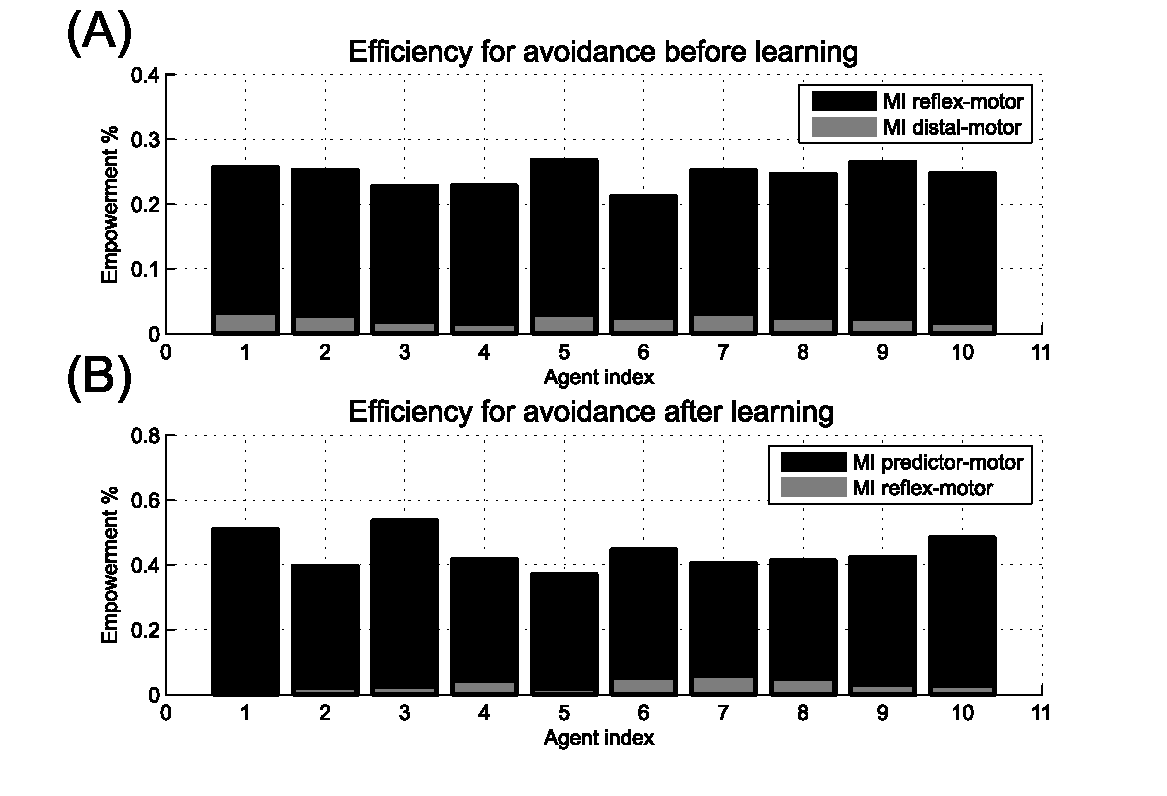
\includegraphics[width=0.8\textwidth]{lawvariety/percentage}
\caption[Information flow and capacity]{
(A) Efficiency for every agent of the reflex-output and predictive-output loop
 in terms of capacity before learning (stage 1):
$MI^4_{Av,U0}/\zeta^4_{all} \%$ (dark bars),
$MI^4_{Av,U1}/\zeta^4_{all}\%$ (grey bars).
(B) Efficiency after learning (stage 3).  \label{fig:Cmax}}
\end{center}
\end{figure}
The $MI$ of order $n=1,2,3$ does not provide enough discrimination for the previous
analysis because the output history of the agent is too short to be correlated with the inputs.
The capacity $\zeta^n_{all}$ takes its maximum of 2 bits when $n \geq 2$.
\subsection{Discussion}
In summary, I have introduced an extension to Ashby's
requisite variety theory called the law of adaptive requisite variety,
computed the information flow to measure the learning performance for agents with
competitive behaviors and found the relation between the efficiency of the information flow $MI$ and the weight change
of the adaptive controller $\Delta \omega_1$.

I also linked the information approach to the Luhmann theory that sub-systems are formed
to reduce the perceived complexity of the environment.
In my simulations, after the learning experience 5 agents have a dominant
attraction behaviour for food disks (seekers) and 5 have a dominant attraction
behaviour for others (parasites).
The seekers mainly use the predictive information of the food disks while the
parasites mainly use the predictive information of the others who posses food.
Thus, my measure of information quantifies the information selection of the agents before and after learning which means I am able to discriminate which agent is a parasite or a seeker without looking at the value of the weights. 

While \citealt{organizationInfo,polaniEmpowerment} and \citealt{LungarellaInformation,Klyubin2008:KeepOptions}
used the empowerment measure as a general cost function to optimise the agent's
behaviour or evolution, I use it as the upper bound of the MI to measure the efficiency of the sensory-motor loop use.
\citet{Ay2008:PredInformation} use an adaptive controller which maximises
the excess entropy (the mutual information
between past and present) at the input side to achieve a working regime exploratory
and sensitive to the environment.
I can calculate the MI for this case by considering the reflex as the present input
and the predictor as the past history.
My approach is not restricted to MISO controllers.
\citet{Kulvicius2009:analysisdifferential} measures the temporal input development, the
output and path entropy of the adaptive agents to study the optimality of the antenna ratio for an avoidance task,
thus completing the tools required to evaluate a single task controller.

The following section \ref{Chapter7:Q learning application} contains some experiment
regarding the application of the mutual information to a Q-learning agent\nomenclature{Q-learning}{Q-learning is a reinforcement learning technique that works by learning an action-value function to predict future rewards} to
verify that this approach is feasible also with reward based learning.
After that, the section \ref{Chapter8:Predictive Performance} introduces a mono-dimensional
measure called Predictive Performance which summarises the learning performance
with a singular scalar measure.
This is necessary to avoid the multi dimensional analysis based on the mutual information
of the predictor and reflex pathway: for every behaviour, like the food attraction,
I have to look at both the values $MI^4_{Fo,U0},MI^4_{Fo,U0}$.
Things get more complicate when it is necessary to compare the performance of 
different agents, because then there is no normalisation basis for doing so.
Another issue is the absolute performance in terms of regulation: how can I identify
if one agent despite its efforts was able to keep its desired state.
These questions will be answered in the section \ref{Chapter8:Predictive Performance}. 



